\chapter{Continuity}\label{chapter:continuity}
If \(f\colon X \to Y\) is a map, the \emph{preimage}\define{preimage} \(f^{-1}S\) of a subset \(S\subseteq Y\) is the set 
\[
f^{-1}S\defeq\set{x\in X|f(x)\in S} \subseteq X.
\]
A \emph{continuous map}\define{continuous} \(f \colon X \to Y\) is a map so that the preimage of any open set in \(Y\) is an open set in \(X\).
\begin{problem}{continuity:usual}
If \(X\) and \(Y\) are subsets of Euclidean space, prove that this agrees with the usual definition.
\end{problem}
Another way to say this: for any point \(x_0 \in X\) and associated point \(y_0 = f\of{x_0}\), if you want \(y=f(x)\) to stay in some neighborhood of the point \(y_0\), you only have to keep \(x\) in a suitable neighborhood of \(x_0\).
Continuity demands precisely that the preimage of a neighborhood is also a neighborhood.
\begin{problem}{continuity:cofinite}
Suppose that \(X\) and \(Y\) are sets equipped with the cofinite topology.
Prove that a map \(f \colon X \to Y\) is continuous just when each point has finite preimage.
\end{problem}
\begin{problem}{continuity:closed.definition}
Prove that a map \(f \colon X \to Y\) is continuous just when the preimage of any closed set is a closed set.
\end{problem}
\begin{problem}{continuity:basis}
We don't need to check \emph{all} open sets: prove that, for any basis \(Y_a \subset Y\) of open sets of a topological space \(Y\), a map \(f \colon X \to Y\) is continuous just when the preimage of any \(Y_a\) is open.
\end{problem}
\begin{problem}{continuity:closure.definition}
Prove that a map \(f \colon X \to Y\) is continuous just when preimage commutes with closure, i.e. for any subset \(A_Y \subset Y\), with closure \(\bar{A}_Y \subset Y\), and with preimage denoted \(A_X=f^{-1}A_Y\), we have \(\bar{A}_X=f^{-1}\bar{A}_Y\).
\end{problem}
\begin{problem*}{continuity:closed.graph}
If \(X\) and \(Y\) are Hausdorff spaces and \(f \colon X \to Y\) is a continuous map, prove that the graph of \(f\) is a closed subset of \(X \times Y\).
\end{problem*}
\begin{problem}{continuity:Zariski}
Prove that every polynomial function \(f \colon \R{n} \to \R{}\) is continuous in the Zariski\SubIndex{Zariski!topology}\SubIndex{topology!Zariski} topologies of \(\R{n}\) and \(\R{}\).
\end{problem}
\begin{problem}{continuity:sin.Zariski}
Prove that the function \(f \colon \R{} \to \R{}\) given by \(f(x)=\sin x\) is discontinuous in the Zariski\SubIndex{Zariski!topology}\SubIndex{topology!Zariski} topology of \(\R{}\).
\end{problem}
\begin{problem}{continuity:exp.Zariski}
Prove that the function \(f \colon \R{} \to \R{}\) given by \(f(x)=e^x\) is continuous in the Zariski\SubIndex{Zariski!topology}\SubIndex{topology!Zariski} topology of \(\R{}\).
\end{problem}
\begin{problem}{continuity:poly.exp.Zariski}
Prove that the function \(f \colon \R{2} \to \R{}\) given by \(f(x,y)=y+e^x\) is discontinuous in the Zariski\SubIndex{Zariski!topology}\SubIndex{topology!Zariski} topology of \(\R{}\).
\end{problem}
\begin{problem}{continuity:constant}
Prove that constant maps are continuous.
\end{problem}
\begin{problem}{continuity:continuous.discrete}
Suppose that \(X\) is a set with the discrete topology, and \(Y\) is any topological space.
What are all continuous maps \(f \colon X \to Y\)?
\end{problem}
\begin{problem}{continuity:continuous.codiscrete}
Suppose that \(X\) is the real number line, and \(Y\) is a set with the discrete topology.
What are all continuous maps \(f \colon X \to Y\)?
\end{problem}
\begin{lemma}
The composition \(g \circ f\) of any continuous maps \(f \colon X \to Y\) and \(g \colon Y \to Z\) is continuous.
\end{lemma}
\begin{proof}
For any open set \(U_Z \subset Z\), note that the set
\[
U_X = \pr{g \circ f}^{-1} U_Z
\]
is just 
\[
U_Z = g^{-1} U_Y
\]
where
\[
U_Y = f^{-1} U_X.
\]
\end{proof}
If \(A \subset X\) is a subset and \(f \colon X \to Y\) is a map, define
\[
\left.f\right|_A \colon A \to Y
\]
by
\[
\left.f\right|_A(a)=f(a)
\]
for every \(a\) in \(A\); the map \(\left.f\right|_A\) is the \emph{restriction}\define{restriction} of \(f\) to \(A\).
\begin{problem}{continuity:restriction}
Prove that the restriction of a continuous map to any set is continuous.
\end{problem}
\begin{problem}{continuity:locality}
Continuity is ``local'': take some open sets \(X_a \subset X\) whose union is \(X\).
Prove that any map \(f \colon X \to Y\) is continuous just when all of its restrictions \(\left.f\right|_{X_a} \colon X_a \to Y\) are continuous.
\end{problem}
\begin{problem}{continuity:very.locality}
Continuity is ``very local''. 
A map \(f \colon X \to Y\) is \emph{continuous at a point} \(x\) in \(X\) if, for any open set \(U_Y \subset Y\) containing \(f(x)\), there is an open set \(U_X \subset X\) containing \(x\) so that \(fU_X \subset U_Y\).
Prove that any map is continuous just when it is continuous at every point.
\end{problem}
\begin{problem}{continuity:projection}
Take topological spaces \(X,Y\) and let \(p \colon X \times Y \to X\) be the map \(p(x,y)=x\), the \emph{projection map}.\define{projection}
Prove that the projection map is continuous.
\end{problem}
\begin{problem}{continuity:binding}
Take topological spaces \(X,Y,Z\) and continuous maps \(f \colon X \to Y\) and \(g \colon X \to Z\) and let \((f,g) \colon X \to Y \times Z\) be \((f,g)(x)=(f(x),g(x))\).
Prove that \((f,g)\) is continuous.
\end{problem}
\begin{problem}{continuity:swap}
Take topological spaces \(X,Y\) and let \(f \colon X \times Y \to Y \times X\) be the map \(f(x,y)=(y,x)\).
Prove that \(f\) is continuous.
\end{problem}
\begin{lemma}
Suppose that \(f, g \colon X \to \R{n}\) are continuous.
Then \(f+g \colon X \to \R{n}\) is continuous.
\end{lemma}
\begin{proof}
Compose \((f,g) \colon X \to \R{n} \times \R{n}\) with the map \(+ \colon \R{n} \times \R{n} \to \R{n}\), continuous maps.
\end{proof}
Similarly, multiplication and division are continuous, etc.
\begin{problem*}{topological:compact.image}
Any continuous map \(f \colon X \to Y\) takes any compact subset \(K \subset X\) to a compact set \(f(K) \subset Y\).
\end{problem*}
\begin{answer}{topological:compact.image}
Take an open cover \(Y_a \subset Y\) of \(f(K)\).
Let \(X_a=f^{-1} Y_a\).
Then \(X_a\) form an open cover of \(f^{-1}f(K)\), and so of \(K\).
Take a finite subcover of \(K\), say \(X_1, X_2, \dots, X_n \subset X\).
Then the corresponding sets \(Y_1, Y_2, \dots, Y_n\) are an open cover of \(f(K)\).
\end{answer}

\section{Density}
The zeroes of a continuous function on \(\R{n}\) form a closed set.
The same is true in much more generality:
\begin{lemma}\label{lemma:continuous.equation}
Take two continuous maps \(f, g \colon X \to Y\).
Let \(A \subset X\) be the set of points at which \(f=g\).
If \(Y\) is Hausdorff, then \(A\) is closed.
\end{lemma}
\begin{proof}
Consider the map \(F \colon X \to Y \times Y\) given by \(F(x)=(f(x),g(x))\).
Let \(\Delta_Y \subset Y \times Y\) be the diagonal, i.e. the set of points of the form \((y,y) \in Y \times Y\) for any \(y \in Y\).
Then clearly \(A=F^{-1}\Delta_Y\). 
By problem~\vref{problem:topology:diagonal}, \(\Delta_Y \subset Y \times Y\) is closed just when \(Y\) is Hausdorff.
So then \(A\) is closed.
\end{proof}
\begin{lemma}
If two continuous maps \(f, g \colon X \to Y\) agree on a dense subset of a Hausdorff space \(X\), then they agree everywhere.
\end{lemma}
\begin{proof}
By lemma~\vref{lemma:continuous.equation}, the set of points where \(f=g\) is closed, so if dense, is \(X\).
\end{proof}

\section{Homeomorphisms}
A \emph{homeomorphism}\define{homeomorphism} is a continuous map \(f \colon X \to Y\) with a continuous inverse \(f^{-1} \colon Y \to X\).
If a homeomorphism \(f \colon X \to Y\) exists, \(X\) and \(Y\) are \emph{homeomorphic}\define{homeomorphic}; for purposes of topology, they are essentially identical.
\begin{example}
The map \(f \colon x \in \R{} \mapsto \arctan x \in (-1,1)\) is a homeomorphism: the real number line is homeomorphic to any open interval of the real number line.
\end{example}
\begin{example}
Let \(X\) be the interval \([0,2 \pi) \subset \R{}\).
Let \(Y\) be the unit circle in the plane \(Y \subset \R{2}\).
The map \(f \colon \theta \in X \mapsto (\cos \theta, \sin \theta) \in Y\) is continuous, and has an inverse \(f^{-1}(\cos \theta, \sin \theta)=\theta\).
But \(f\) is \emph{not} a homeomorphism.
The map \(f^{-1}\) is discontinuous: for points just above the positive horizontal axis, and points just below it, \(f^{-1}\) takes these close points far apart.
To make a proof out of this idea: the \(f^{-1}\) preimage (i.e. the \(f\) image) of the open set \([0,\varepsilon)\) is not open in the circle for \(\varepsilon < 2 \pi\).
\end{example}
\begin{problem}{continuity:ball.to.plane}
Prove that the plane is homeomorphic to any open ball in the plane.
\end{problem}
\begin{theorem}\label{theorem:continuous.bijection}
A continuous bijection \(f \colon X \to Y\) from a compact space \(X\) to a Hausdorff space \(Y\) is a homeomorphism.
\end{theorem}
\begin{proof}
By continuity, open sets have open preimages; equivalently, closed sets have closed preimages.
Closed sets of \(X\) are compact, so their images are compact, so closed: closed sets have closed images.
Equivalently, open sets have open images.
Hence the inverse is continuous.
\end{proof}
\begin{problem}{continuity:ball.to.interval}
Prove that the open unit disk in the plane is not homeomorphic to the real number line.
\end{problem}

\section{Proper maps}
A \emph{proper map}\define{proper!map} \(f \colon X \to Y\) is a continuous map so that the preimage of any compact set is compact.
\begin{problem}{continuity:sine.not.proper}
Which trigonometric and inverse trigonometric functions are proper maps?
\end{problem}
\begin{problem}{continuity:1.point}
The \emph{one point compactification} of a topological space \(X\) is the topological space \(\bar{X}\) whose points are \(X \cup \set{\infty}\) for some element \(\infty\) not in \(X\), and whose open sets are (a) the open sets of \(X\) and (b) the sets \(\set{\infty} \cup (X-C)\) for \(C \subset X\) compact.
Prove that a continuous map \(f \colon X \to Y\) of Hausdorff spaces is proper if and only if it extends to a continuous map \(\bar{f} \colon \bar{X} \to \bar{Y}\) with \(\bar{f}(\infty)=\infty\).
\end{problem}
A map \(f\colon X \to Y\) is \emph{open}\define{open map}\define{map!open} if the image of any open set is open, \emph{closed}\define{closed map}\define{map!closed} if the image of any closed set is closed.
\begin{problem}{continuity:closed.homeo}
Prove that any closed injection \(f\colon X\to Y\) is a homeomorphism to its image.
\end{problem}
\begin{answer}{continuity:closed.homeo}
The image \(f(A)\) of a closed set \(A\subseteq X\) is closed in \(Y\) so closed \(f(X)\).
Hence we can replace \(Y\) by \(f(X)\) and assume the map is a bijection.
Closed sets have closed images.
Open sets have open images by taking complements.
But then for \(f^{-1}\colon Y\to X\), the \(f^{-1}\)-preimages of open sets are just exactly the \(f\)-images, so open.
So \(f^{-1}\) is continuous.
\end{answer}
\begin{problem*}{continuity:proper.test}
A test to decide if a map is proper: prove that a continuous map \(f \colon X \to Y\) is proper if and only if it satisfies the two conditions (a) preimages of points are compact and (b) \(f\) is closed.
\end{problem*}
\begin{answer}{continuity:proper.test}
Suppose (a) and (b).
Pick a compact set \(K\subseteq Y\) and an open cover \(U_{\alpha}\subset X\) of \(f^{-1}K\).
Pick a point \(y_0\in Y\).
Choose finitely many open sets \(U_{\alpha_i}\subseteq X\) covering \(f^{-1}\set{y_0}\); let \(U\) be their union.
Check that \(y_0\) belongs to
\[
W\defeq Y-f(X-U)
\]
which is open since \(f\) is closed.
Note that \(f^{-1}W\subset U\).
For each \(y_0\in Y\), there is some such open set \(W\).
Cover \(K\) by finitely many such \(W\), say \(W_j\), each arising as
\[
W_j=Y-f(X-U_j),
\]
from some open set \(U_j\subset X\) which itself is a finite union of open sets \(U_{\alpha_i}\) on \(X\).
So \(f^{-1}K\) lies inside the union of the various \(f^{-1}W_j\), each of which lies in its \(U_j\).
So \(f^{-1}K\) lies in a finite union of \(U_{\alpha_i}\) sets.
\end{answer}
\begin{problem}{continuity:compact.proper}
Prove that every continuous map \(f\colon X\to Y\) from a compact space to a Hausdorff space is proper.
\end{problem}
\begin{answer}{continuity:compact.proper}
Take a compact set \(K\subseteq Y\).
Since \(Y\) is Hausdorff, \(K\) is closed.
Take an open cover of \(f^{-1}K\) by open sets \(X_a\); add in one more open set \(X_0=X-f^{-1}K\) to give an open cover of \(X\).
Take a finite subcover of \(X\); throw away \(X_0\) to give a finite subcover of \(f^{-1}K\).
\end{answer}
\begin{lemma}\label{lemma:proper.closed}
Every proper map \(f\colon X\to Y\) to a locally compact Hausdorff space \(Y\) is closed.
\end{lemma}
\begin{proof}
Every open set \(U\subseteq Y\) lying in some compact set has compact closure, i.e. is precompact, so \(f^{-1}\bar{U}\) is compact.

Take \(A\subseteq X\) closed.
Pick a point \(y \in Y-f(A)\).
We need only prove there is an open set \(U\) in \(Y\) containing \(y\) avoiding \(f(A)\).
Take any precompact open set \(U\subset Y\) containing \(y\).
Write \(A\) as a union of the compact set \(A'=A\cap f^{-1}\bar{U}\) and the subset \(A''=A\cap f^{-1}(X-\bar{U})\).
Since \(f(A'')\) avoids \(U\), we need only arrange that \(f(A')\) avoids some perhaps smaller open set \(W\) around \(y\), and then \(f(A)\) will avoid \(U\cap W\).
So we can replace \(A\) by \(A'\), \(X\) by \(f^{-1}\bar{U}\), \(Y\) by \(\bar{U}\), so assume both \(X\) and \(Y\) are compact.
By problem~\vref{problem:topological:compact.closed}, \(A\subseteq X\) is compact.
By problem~\vref{problem:topological:compact.image}, \(f(A)\) is compact, and so closed.
\end{proof}

\section{A test for homeomorphism}
\begin{corollary}\label{corollary:proper.bijection}
Take a locally compact Hausdorff space \(Y\).
Any closed injection \(f \colon X \to Y\) is a homeomorphism to its image.
In particular, any proper injection \(f \colon X \to Y\) is a homeomorphism to its image.
\end{corollary}
\begin{proof}
One proof: by lemma~\vref{lemma:proper.closed}, \(f\) is closed; apply problem~\vref{problem:continuity:closed.homeo}.

Another proof, which might give more intuition: write \(Y\) as a union of precompact open sets \(Y_a \subset Y\).
Let \(\bar{X}_a \defeq f^{-1}\bar{Y}_a\).
Then
\[
\left.f\right|_{\bar{X}_a} \colon \bar{X}_a \to \bar{Y}_a
\]
is a homeomorphism to its image by theorem~\vref{theorem:continuous.bijection}.
In particular, if we let \(X_a \defeq f^{-1}Y_a\), then
\[
\left.f\right|_{X_a} \colon X_a \to Y_a
\]
is also a homeomorphism to its image.
Take any open set \(U \subset X\) and let \(U_a \defeq X_a \cap U\).
Then
\[
f(U) = f(\bigcup_a U_a) = \bigcup f(U_a)
\]
is open: open sets have open images.
Hence the inverse is continuous.
\end{proof}

\section{Quotient topologies}
Let's glue things together.
\begin{exampleAndImage}{1cm}
The \emph{M\"obius strip}\define{Moebius strip@M\"obius strip} is given by gluing two sides of a square together, in opposite directions.
Imagine \(X\) is the square, and \(Y\) is the square after we identify those points together; define the map \(X \to Y\) which takes each unglued point to the corresponding point after gluing.
But what is the topology on \(Y\)?
\tcblower
\input{mobius-quotient}
\end{exampleAndImage}
Suppose that we have a map \(f \colon X \to Y\) between two sets \(X\) and \(Y\).
If \(X\) has a topology given, but \(Y\) doesn't, the \emph{quotient topology}%
\define{quotient!topology}%
\define{topology!quotient} on \(Y\) has an open sets precisely those subsets of \(Y\) whose preimages in \(X\) happen to be open.
Clearly for any map \(f \colon X \to Y\), the quotient topology is the ``simplest'' (has the fewest open sets) so that \(f\) becomes continuous.
In a picture, if we draw \(X\) as a looking like a box, and \(Y\) as its shadow on the plane:
\begin{center}

\begin{tikzpicture}
\fill[gray!40] (0,0) rectangle (1,2);
\draw[gray!50,very thick] (0,-.3) -- (1,-.3);
\end{tikzpicture}
\end{center}
and our map takes each point 
\begin{center}

\begin{tikzpicture}
\fill[gray!40] (0,0) rectangle (1,2);
\draw[gray!50,very thick] (0,-.3) -- (1,-.3);
\fill[gray] (.3,1) circle (1.2pt);
\end{tikzpicture}
\end{center}
to its shadow:
\begin{center}

\begin{tikzpicture}
\fill[gray!40] (0,0) rectangle (1,2);
\draw[gray!50,very thick] (0,-.3) -- (1,-.3);
\fill[gray] (.3,1) circle (1.2pt);
\fill[gray] (.3,-.3) circle (1.2pt);
\end{tikzpicture}
\end{center}
then open sets in \(Y\):
\begin{center}

\begin{tikzpicture}
\fill[gray!40] (0,0) rectangle (1,2);
\draw[gray!50,very thick] (0,-.3) -- (1,-.3);
\draw[gray,very thick] (.25,-.3) -- (.6,.-.3);
\draw[gray,fill=white] (.25,-.3) circle (1.2pt);
\draw[gray,fill=white] (.6,-.3) circle (1.2pt);
\end{tikzpicture}
\end{center}
are sets whose preimage is open in \(X\):
\begin{center}
\documentclass[tikz]{standalone}
\begin{document}
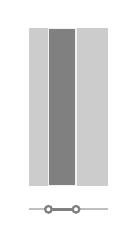
\begin{tikzpicture}
\fill[gray!40] (0,0) rectangle (1,2);
\draw[gray!50,thick] (0,-.3) -- (1,-.3);
\draw[gray,very thick] (.25,-.3) -- (.6,-.3);
\draw[gray,thick,fill=white] (.25,-.3) circle (1.2pt);
\draw[gray,thick,fill=white] (.6,-.3) circle (1.2pt);
\fill[gray,draw=gray!10] (.25,0) rectangle (.6,2);
\end{tikzpicture}
\end{document}
\end{center}
\begin{example}
A \emph{pointed space}\define{pointed space} or \emph{space with marked point}\define{space!with marked point} is a topological space \(X\) together with a point \(x_0\) of \(X\), often denoted \((X,x_0)\).
If \((X,x_0)\) and \((Y,y_0)\) are spaces with marked points, the \emph{join}\define{join} of those spaces is the quotient space \((X \sqcup_{x_0=y_0} Y,x_0)\) defined as follows:
let \(X \sqcup_{x_0=y_0} Y\) be \(X \sqcup Y\) but removing the point \(y_0\).
Map \(f \colon X \sqcup Y \to X \sqcup_{x_0=y_0} Y\) by \(f(x)=x\) but
\[
f(y)=
\begin{cases}
y & \text{ if \(y\ne y_0\)}, \\
x_0 & \text{ if \(y=y_0\)}.
\end{cases}
\]
Give \(X \sqcup_{x_0=y_0} Y\) the marked point \(x_0\) and the quotient topology from this map \(f\).
\end{example}
\begin{exampleAndImage}{1.29cm}
Take \(n\) circles, each with a marked point, and join to get the \emph{bouquet of circles}:\define{bouquet of circles}
\tcblower
\documentclass[tikz]{standalone}
\usepackage{pgfplots}
\usepgfplotslibrary{polar}
\begin{document}
\begin{tikzpicture}
   \clip (0.04,0.115) rectangle (1.33,1.26);
   \begin{polaraxis}[grid=none, axis lines=none,scale=.2]
     \addplot[thick,gray,mark=none,domain=-10:360,samples=300] { abs(cos(6*x/2))};
	\coordinate (centr) at (axis cs:0,0) {};
   \end{polaraxis}
     \fill[gray] (centr) circle (1pt);
 \end{tikzpicture}
\end{document}
\end{exampleAndImage}
\begin{problem}{continuity:metric.quotient}
Prove that if \(f \colon X \to Y\) is a surjective map and \(X\) is a complete metric space and every fiber \(f^{-1}\set{y} \subset X\) of \(f\) is a closed subset, and any two distinct fibers \(f^{-1}\set{y_1}, f^{-1}\set{y_2}\) stay a positive distance apart, then the quotient topology on \(Y\) arises from a metric on \(Y\).
\end{problem}
Another language we use to talk about surjective maps \(f \colon X \to Y\) is the language of equivalence relations.
We can say that two points of \(X\) are equivalent if they have the same value under \(f\).
On the other hand, given an equivalence relation \(\sim\) on \(X\), define the \emph{quotient}\define{quotient} \(X/{\sim}\), to the the set of all equivalence classes, and the \emph{quotient map}%
\define{quotient!map} \(X \to X/{\sim}\) by sending each point \(x \in X\) to its equivalence class \([x]\).
If we write \(X/{\sim}\) as \(Y\) and the quotient map as \(f\) (to avoid the intimidating notation), we define the \emph{quotient topology} by an equivalence relation to be the quotient topology via the quotient map.
It is just a change of notation and language, but we get just the same quotient spaces if we think about surjective maps \(f \colon X \to Y\) or equivalence relations \(\sim\) on a topological space \(X\).
\begin{theorem}
Take a topological space \(X\) and an equivalence relation \(\sim\) on \(X\) with quotient map \(X \to X/{\sim}\).
Any continuous map \(X/{\sim} \to Y\) induces a continuous map \(X \to Y\) by composing with the quotient map: \(X \to X/{\sim} \to Y\).

Conversely, a continuous map \(X \to Y\) arises in this way, i.e. has the form of a composition \(X \to X/{\sim} \to Y\), for a unique continuous map \(X/{\sim} \to Y\) just when it is constant on equivalence classes, i.e. equivalent elements go to the same point of \(Y\).
We then say that that our map \(X \to Y\) \emph{descends to the quotient}.
\end{theorem}
\begin{proof}
Suppose that \(f \colon X \to Y\) is a continuous map taking equal values in \(Y\) for any equivalent points of \(X\).
We define a map, perhaps not continuous, by \(\bar{f}([x])=f(x)\) on each equivalence class \([x] \in X/{\sim}\).
Clearly this is well defined, but we need to prove that it is continuous.
Let \(q \colon X \to X/\sim\) be the quotient map taking each point \(x \in X\) to its equivalence class \([x] \in X/\sim\).
Note also that by definition \(f(x)=\bar{f}([x])\), i.e. \(f=\bar{f} \circ q\).
Take an open set \(U_Y \subset Y\).
Take its preimage \(U_{X/{\sim}} \subset X/{\sim}\).
We need to prove that \(U_{X/{\sim}} \subset X/{\sim}\) is open.
By definition of the quotient topology, this is precisely proving that \(U_X \defeq q^{-1}U_{X/{\sim}}\) is open.
But this is just
\begin{align*}
U_X
&=
q^{-1} \bar{f}^{-1} U_Y,
\\
&= \pr{\bar{f} \circ q}^{-1} U_Y,
\\
&=
f^{-1} U_Y,
\end{align*}
open in \(X\).
\end{proof}
\begin{problem}{continuity:quotient.compact}
Suppose that \(f \colon X \to Y\) is a surjective map from a topological space \(X\).
Suppose that \(X\) contains a compact set \(K\) for which \(f(K)=Y\).
Prove that \(Y\) is compact in the quotient topology.
\end{problem}
\begin{problem}{continuity:open.map}
A map \(f\colon X \to Y\) is \emph{strict}\define{strict map}\define{map!strict} if the induced topology on \(f(X)\) agrees with the quotient topology.
Prove that every surjective open map is strict, and that every surjective closed map is strict.
\end{problem}
Often we can guess what the quotient space by a map should be, and we need the following theorem to check our guess.
\begin{theorem}
Suppose that \(f \colon X \to Y\) is a continuous surjective map and \(Y\) is Hausdorff.
Suppose that every point of \(Y\) lies in the interior of the image of a compact subset of \(X\).
Define an equivalence relation: \(x_1 \sim x_2\) just when \(f(x_1)=f(x_2)\) for any \(x_1, x_2\) in \(X\).
Then \(f \colon X \to Y\) descends to the quotient to a homeomorphism \(X/{\sim} \to Y\).
\end{theorem}
\begin{proof}
Clearly the quotient map \(X/{\sim} \to Y\) is a bijection and constant on equivalence classes, so continuous.
Pick an open subset \(U_Y \subset Y\), which lies in the image of some compact set \(K_X \subset X\).
We can replace \(K_X\) by its intersection with the preimage of \(\bar{U}_Y\), so that \(f(K_X)=\bar{U}_Y\).
By problem~\vref{problem:topological:compact.image}, the image of \(K_X\) in \(K_{X/{\sim}} \subset X/{\sim}\) is compact.
By theorem~\vref{theorem:continuous.bijection}, \(K_{X/{\sim}} \cong \bar{U}_Y\) is a homeomorphism.
So near each point of \(Y\), the quotient map is a homeomorphism.
\end{proof}
\begin{problem*}{continuity:quotient.On}
Suppose that \(f\) is a continuous function
\[
f(v_1,v_2,\dots,v_n)
\]
of vector variables \(v_j\in\R{n}\).
Suppose that \(f\) is invariant under simultaneous orthogonal transformation of all of the vectors:
\[
f(Uv_1,Uv_2,\dots,Uv_n)=f(v_1,v_2,\dots,v_n),
\]
for any orthogonal \(n\times n\) matrix \(U\).
Let \(Y\) be the set of all positive semidefinite symmetric matrices, i.e. symmetric matrices \(A\) so that \(\ip{Av,v}\ge 0\) for any vector \(v\in\R{n}\).
Prove that there is a continuous function \(g\colon Y \to\R{}\) so that \(f\) can be written as 
\[
f(v_1,v_2,\dots,v_n)=g(A)
\]
where \(A\) is the matrix with entries \(A_{ij}=\ip{v_i}{v_j}\).
\end{problem*}
\begin{answer}{continuity:quotient.On}
The firs problem is to use linear algebra to prove that any matrix \(A\in Y\) arises as a \emph{Gram matrix}
\[
A=\varphi(v_1,\dots,v_n),
\]
where \(\varphi\) is the map giving \(A_{ij}=\ip{v_i}{v_j}\).
For this, you can use induction on dimension.
The second problem is to show that this Gram matrix uniquely determines the vectors \(v_1,\dots,v_n\) up to orthogonal linear transformation.
Hence the map \(\varphi\) associating to vectors their Gram matrix is an injection modulo the action of the orthogonal group.
The third problem is to prove that every point \(A\in Y\) lies in the interior of the image of a compact set of choices of vectors \(v_1,\dots,v_n\); but this follows from taking all of the vectors to lie in some large enough ball in \(\R{n}\), so that every Gram matrix whose diagonals are bounded by the radius of that ball lies in the image of that set.
\end{answer}
\begin{problem}{continuity:make.quot}
Suppose that \(\mathcal{B}\) is a collection of open subsets of a topological space \(X\).
Suppose that, for any \(U,V\in\mathcal{B}\), and point \(x\in U\cap V\), there is an open set \(W\in\mathcal{B}\) so that \(x\in W\subseteq U\cap V\).
Prove that there is a topological space \(Y\) and an onto continuous map \(f\colon X \to Y\) so that \(f\) takes every set \(U\in\mathcal{B}\) to an open set \(f(U)\), and \(f^{-1}f(U)=U\), and these sets \(f(U)\) form a basis of open sets of \(Y\).
\end{problem}
If \(A \subset X\) is a subset of a topological space, \(X/A\) means the quotient where we make any two points of \(A\) equivalent, and no other points equivalent to one another.
If \(X\) is a metric space and \(A\) is closed then \(X/A\) is also a metric space, so we have an enormous collection of examples of metric spaces.
\begin{problem}{continuity:build.circle}
Let \(X\) be the closed unit interval \([0,1] \subset \R{}\) and \(Y\) the unit circle in the plane.
Let \(f \colon X \to Y\) by \(f(x)=(\cos 2\pi x, \sin 2\pi x)\).
Prove that \(X/\set{0,1}\) is homeomorphic to \(Y\).
\end{problem}
\begin{problem*}{continuity:build.sphere}
Let \(X\) be the closed unit ball \(X=\bar{B} \subset \R{}\) and \(Y \subset \R{n+1}\) the unit sphere.
Let \(A \subset X\) be the unit sphere.
Write points of \(\R{n+1}\) as \((t,x)\) for \(t \in \R{}\) and \(x \in \R{n}\).
Consider the map \(f \colon X \to Y\) given by
\[
f(x)=
\begin{cases}
\left(\cos(\pi |x|), \sin(\pi |x|)\frac{x}{|x|}\right), & \text{ if \(|x|\ne 0\)}, \\
(1,0), & \text{ if \(|x|=0\).}
\end{cases}
\]
Prove that \(f\) is continuous.
Prove that \(f\) is injective from the interior of \(X\) to \(Y-\set{(-1,0)}\) and that \(f\) takes every point of \(A\) to the point \((-1,0) \in Y\).
Prove that \(X/A\) is homeomorphic to \(Y\).
\end{problem*}
\begin{answer}{continuity:build.sphere}
  If we let \(t=\pi |x|\) then \(|f(x)|^2=\cos^2 t + \sin^2 t=1\), so \(f\) is valued in the unit sphere \(Y\).
  Continuity is clear except when \(|x| \to 0\), but then the fact that \(\sin' t=\cos t\) tells us that
  \[
  \frac{\sin t}{t} 
  \]
  is continuous with
  \[
  1 = \lim_{t \to 0} \frac{\sin t}{t}
  \]
  by L'Hôpital's rule.
  Write
\[
f(x)=
\begin{cases}
\left(\cos(\pi |x|), \frac{\sin(\pi |x|)}{|x|}x\right), & \text{ if \(|x|\ne 0\)}, \\
(1,0), & \text{ if \(|x|=0\).}
\end{cases}
\]
to see that \(f(x) \to (1,0)\) as \(|x| \to 0\), continuity.
  Clearly \(f(0)=(1,0)\) and, if \(|x|=1\), then \(f(x)=(-1,0)\).
  Since \(0 \le \pi|x| \le 1\),  if \(f(x)=(-1,0)\) then \(\cos(\pi|x|)=-1\) and \(\sin(\pi|x|)=0\) and so \(\pi|x|=\pi\), i.e. \(|x|=1\).
  If \(x, y \in X\) and \(|x|<1\) and \(|y|<1\) and if \(f(x)=f(y)\) then
  \[
  \cos(\pi|x|)=\cos(\pi|y|)
  \]
  so \(0\le |x|=|y| < 1\).
  But then also
  \[
  \sin(\pi|x|)x=\sin(\pi|y|)y
  \]
  and \(\sin(\pi|x|) \ne 0\) so \(x=y\).
  Hence \(f\) is continuous and 1-1.
  Since \(X\) is compact and \(Y\) is Hausdorff and \(f\) is onto, \(f\) identifies \(Y\) with the quotient of \(X\) by the map, i.e. with the closed ball with its boundary glued to a single point.
\end{answer}
\begin{exampleAndImage}{1cm}
The \emph{M\"obius strip}\define{Moebius strip@M\"obius strip} is the quotient of the closed unit square \(X=[0,1] \times [0,1]\) by the equivalence relation \((0,y)\sim(1,1-y)\):
\tcblower
\input{mobius-quotient}
\end{exampleAndImage}
\begin{exampleAndImage}{1cm}
The \emph{Klein bottle}\define{Klein bottle} is the quotient of the closed unit square \(X=[0,1] \times [0,1]\) by the equivalence relation \((x,0)\sim(x,1)\) and \((0,y)\sim(1,1-y)\):
\tcblower
\input{klein-quotient}
\end{exampleAndImage}
\begin{exampleAndImage}{1cm}
The torus is the quotient of the closed unit square \(X=[0,1] \times [0,1]\) by the equivalence relation \((x,0)\sim(x,1)\) and \((0,y)\sim(1,y)\).
\tcblower
\documentclass[tikz]{standalone}
\usetikzlibrary{decorations.markings}
\begin{document}
\begin{tikzpicture}
\fill[draw=gray,gray!50] (0,0) rectangle (1,1);
\begin{scope}[very thick,decoration={
    markings,
    mark=at position 0.5 with {\arrow{latex}}}
    ] 
    \draw[postaction={decorate},thick,gray] (0,0) -- (0,1);
    \draw[postaction={decorate},thick,gray] (1,0) -- (1,1);
\end{scope}
\begin{scope}[very thick,decoration={
    markings,
    mark=at position 0.5 with {\arrow{>>}}}
    ] 
    \draw[postaction={decorate},thick,gray] (0,0) -- (1,0);
    \draw[postaction={decorate},thick,gray] (0,1) -- (1,1);
\end{scope}
\end{tikzpicture}
\end{document}

\end{exampleAndImage}
\begin{example}
The \emph{real projective space}\define{real!projective space} is the quotient \(\RP{n}=S^n/(x \sim -x)\).
Every line through the origin strikes the unit sphere at two antipodal points.
In other words, a point of real projective space corresponds to a line through the origin in \(\R{n+1}\).
\end{example}
\begin{example}
The \emph{complex projective space}\define{complex!projective space} is the quotient \(\CP{n}=\RP{2n+1}/\sim\) where a unit length vector \(z \in \C{n+1}\) is equivalent to \(e^{i \theta} z\) for any real number \(\theta\).
In other words, a point of complex projective space corresponds to a complex line through the origin in \(\C{n+1}\).
\end{example}
\begin{example}
The \emph{quaternionic projective space}\define{quaternionic projective space} is the quotient \(\HP{n}=\CP{2n+1}/\sim\) where a unit length vector \(z \in \Quat{n+1}\) is equivalent to \(\lambda z\) for any unit length quaternion \(\lambda\).
In other words, a point of quaternionic projective space corresponds to a quaternionic line through the origin in \(\Quat{n+1}\).
\end{example}
\begin{exampleAndImage}{2cm}
Let \(\bar{D}\) be the closed unit disk, i.e. the set of points \((x,y)\) so that \(x^2+y^2\le 1\).
The map
\[
(x,y)\in\bar{D}\mapsto(x,y,z(x,y))
\]
where
\[
z(x,y)=\sqrt{1-x^2-y^2}
\]
parameterizes precisely the top half of the unit sphere, the upper hemisphere.

Let \(\pi\colon S^2\to\RP{2}\) be the quotient map, taking each unit vector \((x,y,z)\) to the line through that vector and the origin, i.e. quotienting by \((x,y,z)\sim-(x,y,z)\).
Consider the map
\[
f\colon(x,y)\in\bar{D}\mapsto\pi(x,y,z(x,y)).
\]
This map is onto, as every line through the origin strikes a point of the upper hemisphere.
But horizontal lines strike the equator twice at opposite points.
So \(f\) is not injective; indeed \(f\) is injective precisely in the interior of the disk, and \(2\) to \(1\) along the boundary of the disk, taking \((x,y)\) and \((-x,-y)\) on the unit circle to the same line: the one spanned by \((x,y,0)\).
Define an equivalence relation \(\sim\): two points are equivalent if their images are the same under \(f\).
The map \(f\) descends to a homeomorphism \(\bar{D}/\sim\cong\RP{2}\), since \(\bar{D}\) is compact, and \(f\) is surjective, every point of \(\RP{2}\) lies in the interior of the image of \(\bar{D}\).
\tcblower
\begin{tabular}{c}
\documentclass[tikz]{standalone}
\usepackage{graphics}
\begin{document}
\begin{tikzpicture}
\node[anchor=south west,inner sep=0] at (0,0) {\includegraphics[width=2cm]{hemisphere.pdf}};
\draw  (.5,.75)--(.5,1.15);
\fill (.5,.75) circle (.8pt);
\fill (.5,1.15) circle (.8pt);
\end{tikzpicture}
\end{document}\\[4cm]
\documentclass[tikz]{standalone}
\usetikzlibrary{decorations.markings}
\begin{document}
\begin{tikzpicture}
\fill[draw=gray,gray!50] (0,0) circle (.5cm);
\begin{scope}[very thick,decoration={
    markings,
    mark=at position 0.5 with {\arrow{latex}}}
    ] 
%    \draw[postaction={decorate},thick,gray] (0,0) circle (1cm);
    \draw[rotate=90,postaction={decorate},thick,gray] (0,0) circle (.5cm);
%  \draw[rotate=180,postaction={decorate},thick,gray] (0,0) circle (1cm);
    \draw[rotate=270,postaction={decorate},thick,gray] (0,0) circle (.5cm);
\end{scope}
\end{tikzpicture}
\end{document}

\end{tabular}
\end{exampleAndImage}